\documentclass[11pt,a4paper]{article}
\usepackage[margin=2.7cm]{geometry}
\usepackage{amsmath,amssymb,amsthm,booktabs,tikz,microtype,float}
\usepackage[colorlinks,linkcolor=black,citecolor=black,urlcolor=blue!50!black]{hyperref}

\definecolor{curveC}{HTML}{111111}\definecolor{squareC}{HTML}{D1342F}
\definecolor{discC}{HTML}{2A7DE1}\definecolor{looseC}{HTML}{B9770E}

\newtheorem{conjecture}{Conjecture}
\theoremstyle{definition}\newtheorem{definition}{Definition}
\theoremstyle{remark}\newtheorem{remark}{Remark}

\title{The trapped ball:\\ a conjecture on the size of inscribed squares}
\author{Olli Paloviita}
\date{November 2026}

\begin{document}
\maketitle

\begin{abstract}
The largest disc inside a polygon does not bound the size of its inscribed
squares from below~\cite{small}. We propose a quantity that might: the radius
$r^*$ of the largest disc that can still be moved between any two places where
it fits inside the polygon. For a convex polygon this is the inradius; for a
polygon with a narrow doorway it is half the width of the doorway. We conjecture
that every simple polygon has an inscribed square of side at least
$\sqrt2\,r^*$, the value attained by the circle. The conjecture is not proved.
It holds for every polygon we tried, including all known examples whose squares
are small compared with the inradius, and direct computer searches for a
counterexample, over more than seven million polygons, ended at $\sqrt2$ to
four figures. Put the other way round: the only way to make all inscribed
squares of a polygon small would be to give it a narrow doorway.
\end{abstract}

\noindent\textbf{Status.} This note states a guess and the numerical evidence
for it. It proves nothing. The author is a software developer, not a
mathematician; the experiments and this text were produced by guiding coding
agents. The inscribed squares are computed exactly, the other quantities in
floating point. As far as we know the statement is new. The table in
Section~\ref{sec:evidence} can be reproduced from
\url{https://github.com/ollipal/small-inscribed-squares}; the searches cannot.

\section{The question}

A square is \emph{inscribed} in a closed curve if its four corners lie on the
curve. Every polygon has an inscribed square, and it is open whether every
Jordan curve has one. One would like to approximate a curve by polygons and pass
to the limit, which works as soon as the squares of the approximating polygons
are prevented from shrinking to a point; Greene and Lobb~\cite{gl} call this
obstacle \emph{shrinkout}. The folklore \emph{big peg conjecture}
proposed that the inradius prevents it: a polygon containing a disc of radius
$\rho$ should have an inscribed square of side at least $\varepsilon\rho$
\cite{matschke-survey,schwartz}. In its sharp form, posed by
Bernier~\cite{bernier}, the constant would be $\sqrt2$, the value for a circle.

Both forms are false. Szab\'o and Schwartz~\cite{ss} found polygons with $5$ to
$9$ sides whose largest inscribed square has side about $1.14\,\rho$, and
Pochuev~\cite{pochuev} a $10$-gon at $1.41\,\rho$, below $\sqrt2$. The companion
paper~\cite{small} gives $13$-gons $P(m)$ with $\rho\ge 2m$ whose only inscribed
square has side less than $37$, so no $\varepsilon>0$ works.

In $P(m)$ three large rooms meet at a small hub. Each room's large squares need a
corner in the doorway to the hub, and are lost. What remains is one square the
size of the hub. This suggests that the squares of a polygon answer not to its
largest disc but to its narrowest doorway: that the only way to make all
inscribed squares small is to give the polygon a narrow doorway. The next
section makes that a number.

\paragraph{Related work.} We did not find the quantity $r^*$ or
Conjecture~\ref{conj} in the literature; the size statements we found all use
the inradius. Two results are close in spirit. Schulz~\cite{schulz} shows that
an inscribed square of side less than $\sqrt2\,\rho$ must have a corner hidden
behind the convex hull of the disc and the other three corners, in a pocket of
the curve; this constrains each small square but does not bound the largest.
Cantarella, Denne and McCleary~\cite{cdm} bound every square inscribed in a
curve of finite total curvature without cusps from below by a distance defined
through the curvature of short arcs; that quantity is small as soon as the curve
has a small bump. Proved lower bounds for the largest square are known for
curves in an annulus (Matschke), for convex curves (see Section~\ref{sec:weak}) and
for pairs of Lipschitz graphs (Rifford~\cite{rifford}).

\section{The trapped ball}

Let $P$ be a simple polygon with interior $D$, and for $x\in D$ let $d(x)$ be the
distance from $x$ to the boundary. For $r>0$ put
\[
  D_r=\{x\in D : d(x)\ge r\},
\]
the set of positions available to the centre of a disc of radius $r$ inside $P$.
The inradius is $\rho=\max d$.

\begin{definition}
$r^*(P)$ is the supremum of the $r\in(0,\rho]$ such that $D_s$ is connected for
every $s\le r$.
\end{definition}

For small $s$ the set $D_s$ is connected. As $s$ grows it may fall into several
pieces: a disc of radius $s$ placed in one piece cannot be moved into another,
and we say that it is \emph{trapped}. So $r^*$ is the radius at which a disc is
first trapped, and $r^*=\rho$ if that never happens.

\begin{itemize}
\item If $P$ is convex then every $D_s$ is convex, so $r^*=\rho$.
\item For the polygons $P(m)$ of~\cite{small}, $D_s$ falls into pieces when $2s$
exceeds the width of the doorway between two rooms. Hence $r^*=5.30$ for every
$m$, while $\rho$ grows like $3m$ (Table~\ref{tab}).
\item A disc is first trapped at a \emph{pinch}: a segment from a reflex corner
of $P$ to another reflex corner, or to the nearest point of a side, with no
boundary point closer to its midpoint than its two ends, and with a disc of
larger radius fitting on either side of it. Then $r^*$ is half the length of the
shortest pinch. This is how $r^*$ is computed here.
\end{itemize}

\begin{figure}[H]\centering
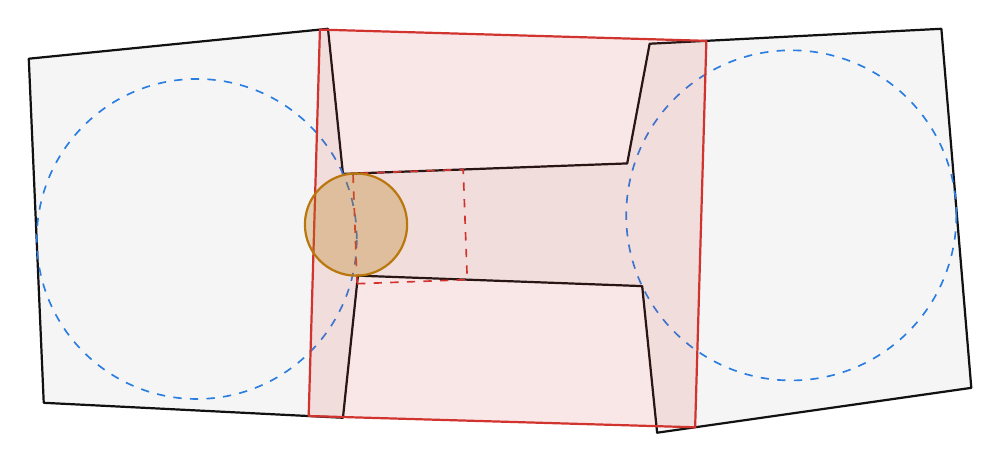
\begin{tikzpicture}[x=1.9cm,y=1.9cm,line join=round]
\path[draw=curveC, line width=0.8pt, fill=black!4] (-3.0000,-1.2000) -- (-1.0000,-1.3000) -- (-0.9000,-0.3500) -- (1.0000,-0.4200) -- (1.1000,-1.4000) -- (3.2000,-1.1000) -- (3.0000,1.3000) -- (1.0500,1.2000) -- (0.9000,0.4000) -- (-1.0000,0.3300) -- (-1.1000,1.3000) -- (-3.1000,1.1000) -- cycle;
\path[draw=discC, dashed, line width=0.6pt] (1.9968,0.0528) circle (1.1033);
\path[draw=discC, dashed, line width=0.6pt] (-1.9771,-0.1049) circle (1.0695);
\path[draw=squareC, line width=0.8pt, fill=squareC, fill opacity=0.12] (-1.2291,-1.2885) -- (1.3541,-1.3637) -- (1.4292,1.2194) -- (-1.1539,1.2946) -- cycle;
\path[draw=squareC, dashed, line width=0.6pt] (-0.9057,-0.4041) -- (-0.1692,-0.3769) -- (-0.1963,0.3596) -- (-0.9328,0.3325) -- cycle;
\path[draw=looseC, line width=0.8pt, fill=looseC, fill opacity=0.3] (-0.9126,-0.0086) circle (0.3416);
\end{tikzpicture}

\caption{A $12$-gon with two rooms and a corridor. Dashed: the largest discs
that fit, $\rho=1.11$. Shaded disc: the largest that is not trapped,
$r^*=0.34$, sitting on the pinch. Square: the largest of the eleven inscribed
squares, side $0.74$. Here $S/\rho=0.66$ and $S/r^*=2.16$.}\label{fig}
\end{figure}

\section{The conjecture}

Write $S(P)$ for the side of the largest inscribed square of $P$.

\begin{conjecture}\label{conj}
For every simple polygon $P$, \quad $S(P)\ \ge\ \sqrt2\; r^*(P)$.
\end{conjecture}

\begin{remark}
The constant cannot be larger: a polygon approximating a circle has
$r^*=\rho$ and $S\to\sqrt2\,\rho$. Among the polygons found by the searches of
Section~\ref{sec:evidence}, the extremal ones have an inscribed circle that
touches the polygon at the four corners of a square.
\end{remark}

\begin{remark}
Conjecture~\ref{conj} is the sharp big peg conjecture with $\rho$ replaced by
$r^*$. Since $r^*\le\rho$ it is weaker, and the counterexamples to the original
do not contradict it: in each of them a disc is trapped.
\end{remark}

\begin{remark}
A slightly stronger inequality held in every polygon we evaluated ($152$
polygons, smallest ratio $1.000004$): $S\ge\min(\sqrt2\,\rho,\;2r^*)$. In words,
the largest square is at least as wide as the narrowest pinch, unless
$\sqrt2\,\rho$ is smaller. It is attained by the ring octagon of~\cite{small}
and by a pentagon of~\cite{ss}. We did not search for counterexamples to it.
\end{remark}

\begin{remark}
Stated the other way round: the only way to make all inscribed squares of a
polygon small is to give it a narrow doorway.
\end{remark}

\section{Evidence}\label{sec:evidence}

\subsection*{Known polygons}

Table~\ref{tab} lists $S$, $\rho$ and $r^*$ for ten polygons. $S$ is exact
(\texttt{verify.py}, complete enumeration in rational arithmetic); $\rho$ and
$r^*$ are floating point (\texttt{trapped\_ball.py}).

\begin{table}[H]\centering\small
\begin{tabular}{lrrrrrr}
\toprule
Polygon & sides & $S$ & $\rho$ & $r^*$ & $S/\rho$ & $S/r^*$\\
\midrule
regular pentagon & 5 & 1.2467 & 0.8090 & 0.8090 & 1.541 & 1.541\\
a kite & 4 & 0.7748 & 0.5180 & 0.5180 & 1.496 & 1.496\\
two rooms and a corridor (Figure~\ref{fig}) & 12 & 0.7370 & 1.1109 & 0.3416 & 0.663 & 2.158\\
pentagon of \cite[Appendix]{small} & 5 & 2.5686 & 1.8856 & 1.2728 & 1.362 & 2.018\\
ring octagon of \cite[\S4]{small} & 8 & 7.2801 & 5.2565 & 3.6401 & 1.385 & 2.000\\
Pochuev's $10$-gon \cite{pochuev}, scaled by 1200 & 10 & 1692.5 & 1201.2 & 840.3 & 1.409 & 2.014\\
$P(20)$ & 13 & 35.99 & 60.7 & 5.303 & 0.593 & 6.79\\
$P(40)$ & 13 & 33.06 & 120.6 & 5.303 & 0.274 & 6.23\\
$P(80)$ & 13 & 31.73 & 240.7 & 5.303 & 0.132 & 5.98\\
an extremal polygon from the search & 8 & 114.79 & 81.16 & 81.16 & 1.414 & 1.4143\\
\bottomrule
\end{tabular}
\caption{The old measure $S/\rho$ and the new one $S/r^*$. The first tends to
$0$ along $P(m)$; the second is never below $\sqrt2=1.4142$.}\label{tab}
\end{table}

The five polygons with explicit coordinates in the correspondence~\cite{ss} were
also evaluated. Each has exactly one inscribed square and each has a pinch. Our
values of $S/\rho$ are $1.144$, $1.208$, $1.176$, $1.161$ and $1.135$, which
reproduce the ratios reported there; the values of $S/r^*$ are $2.000$, $2.002$,
$5.44$, $2.000$ and $2.000$. In four of the five the pinch is a side of the
inscribed square.

\subsection*{Searches}

The following were computer searches by simulated annealing over polygons with
at most $26$ sides, the objective evaluated in floating point by complete
enumeration of the inscribed squares. Reported polygons were then enumerated
exactly. Together the searches evaluated more than seven million polygons; the
first alone visited about $7.8$ million.

\begin{itemize}
\item \emph{Pushing the square below the doorway.} With the rooms of $P(40)$
fixed, the hub was decorated with features down to $1/130$ of the original
square. $S$ fell from $33.06$ to about $5.0$ and stayed there. Requiring the
walls to stay a distance $w$ apart gave $S=1.0003\,w$ and $S=1.0004\,w$ for
$w=10.6$ and $5.8$. In about $7.8$ million polygons visited there was always a
square with corners on two different walls, never smaller than the gap.
\item \emph{Minimising $S/r^*$.} From random polygons, a star, an L, a spiral
strip, a dumbbell and hubs with $3$, $4$ and $5$ rooms, every valid run
ended between $1.4142$ and $1.4147$. Runs started from three-room polygons
stayed at $2.000$.
\item \emph{Between the two regimes.} Thirteen starts with a dent that nearly
traps a disc (dumbbells with wide corridors, overlapping discs, dented discs and
squares). The smallest value was $S/\rho=1.41421\pm0.00002$ on a $16$-gon whose
one inscribed square is inscribed in its inscribed circle. For two overlapping
unit discs with centres $c$ apart, $S/r^*$ increases with $c$ from $1.51$ to
$6.3$, continuously through the value of $c$ at which a disc becomes trapped.
\end{itemize}

\subsection*{Small pinches}

A thin arm that widens slightly towards its end is a pinch like any other, and
$r^*$ takes it into account. Such pinches usually have a small inscribed square
at them: of $344$ pinches in $200$ random polygons, $340$ had a square at least
as wide as the pinch nearby. It is not forced: $P(40)$ has three pinches and a
single square. Rules that disregard small pinches lose the constant $\sqrt2$:
they fail on a pentagon of~\cite{ss}, where the two sides of the pinch are
almost equally roomy, and on a $24$-gon found by search.

\section{What is weak}\label{sec:weak}

\begin{itemize}
\item \emph{Without a pinch it is the sharp bound for that class.} When no disc
is trapped the conjecture says $S\ge\sqrt2\,\rho$. For convex curves this bound
has been reported (C.~Boilley, 2026; see the research log~\cite{schulz}). For
polygons that are not convex but have no pinch, such as an L or a star, it is
not known. The support there is that every polygon known to us with
$S<\sqrt2\,\rho$ has a pinch.
\item \emph{The evidence is computer search.} The searches were carried out with
the help of coding agents, on polygons with at most $26$ sides, with the aim of
finding a counterexample. None was found; that is not a proof.
\item \emph{It would not settle the inscribed square problem.} A Jordan curve
can have pinches at every scale; then $r^*=0$ and nothing is claimed.
\end{itemize}

\section{Reproducing the table}

\begin{verbatim}
python3 trapped_ball.py                  # Table 1, about 15 seconds
python3 trapped_ball.py "x,y;x,y;..."    # any polygon
\end{verbatim}
Python~3, standard library only. The search programs are not part of the
repository.

\begin{thebibliography}{9}\small
\bibitem{bernier} D.~Bernier, \emph{The sharp big peg conjecture}, 16 June 2026,
\url{https://dbernier.ca/2026/06/16/the-sharp-big-peg-conjecture/}.
\bibitem{cdm} J.~Cantarella, E.~Denne and J.~McCleary, Square-like quadrilaterals
inscribed in embedded space curves, \href{https://arxiv.org/abs/2103.13848}{arXiv:2103.13848}.
\bibitem{gl} J.~Greene and A.~Lobb, Floer homology and square pegs,
\href{https://arxiv.org/abs/2404.05179}{arXiv:2404.05179}.
\bibitem{matschke-survey} B.~Matschke, A survey on the square peg problem,
Notices Amer.\ Math.\ Soc.\ 61 (2014), 346--352.
\bibitem{small} O.~Paloviita, \emph{Inscribed squares can be small: a
counterexample to the big peg conjecture} (2026),
\url{https://github.com/ollipal/small-inscribed-squares}.
\bibitem{pochuev} G.~Pochuev, \emph{A 10-vertex counterexample to David
Bernier's sharp polygonal big peg conjecture} (2026),
\url{https://github.com/Grisha-Pochuev/sharp-big-peg-counterexample}.
\bibitem{rifford} L.~Rifford, A quantitative version of Tao's result on the
Toeplitz square peg problem, \href{https://arxiv.org/abs/2106.01914}{arXiv:2106.01914}.
\bibitem{schulz} B.~J.~Schulz, \emph{Toeplitz square-peg research}, software repository (2026),
\url{https://github.com/HiroSakuraba/Toeplitz.-Round-peg}.
\bibitem{ss} R.~E.~Schwartz and Z.~Szab\'o, with J.~Greene and A.~Lobb,
correspondence of 31 May -- 2 June 2026, communicated by R.~E.~Schwartz,
26 November 2026, and cited with his permission.
\bibitem{schwartz} R.~E.~Schwartz, Rectangles, curves, and Klein bottles,
Bull.\ Amer.\ Math.\ Soc.\ 59 (2022), 1--17.
\end{thebibliography}
\end{document}
